%
% Implicit Learning
%

\section{Implicit Learning Deficits in Autism}

%Investigations into implicit learning in autism have led some researchers to suggest a general deficit in this domain.  Poor performance on tasks such as the learning of artificial grammars~\cite{RefWorks:147} and an apparent lack of learning during serial response time tasks (SRTT) have been used in support of this conjecture~\cite{RefWorks:148,RefWorks:149}.  A proposed computational exploration of the behavioral data utilizing the SRTT will be completed as part of this research project.  

%In addition to executive dysfunction and stimulus overselectivity, is it plausible that abnormal PFC/DA interactions can also account for the deficits in implicit learning observed in people with autism?  Implicit learning is learning that occurs without any awareness of the specific knowledge acquired during the process.  Researchers have suggested that people with autism have a core deficit in their ability to implicitly learn about the inherent relationships that exist between objects and situations in the world~\cite{RefWorks:148,RefWorks:149}.  Klinger et al. argue that impaired implicit learning results in difficulties in recognizing the relationships that exist across experiences, likely leading to problems forming general knowledge about categories of items and types of situations.  Difficulties in generalizing learned knowledge to new situations are commonly observed in people with autism, and these difficulties frequently act as a central obstacle to the development of behaviors needed for autonomy and independent living.  Thus, a precise characterization of the mechanisms responsible for these generalization deficits would be very valuable to any effort to design ways to mitigate these serious issues in people with autism.

Researchers have suggested that people with autism have a core deficit in their ability to implicitly learn about the inherent relationships that exist between objects and situations in the world~\cite{RefWorks:148,RefWorks:149}.  Klinger et al. argue that impaired implicit learning results in difficulties in recognizing the relationships that exist across experiences, likely leading to problems forming general knowledge about categories of items and types of situations.  Difficulties in generalizing learned knowledge to new situations are commonly observed in people with autism, and these difficulties frequently act as a central obstacle to the development of behaviors needed for autonomy and independent living.  Thus, a precise characterization of the mechanisms responsible for these generalization deficits would be very valuable to any effort to design ways to mitigate these serious issues in people with autism.

\subsection{The Serial Response Time Task (SRTT)}
Poor performance on tasks such as the learning of artificial grammars~\cite{RefWorks:147} and an apparent lack of learning during serial response time tasks (SRTT) have been used as evidence supporting implicit learning deficits in people with ASD~\cite{RefWorks:148,RefWorks:149}.  In the following we specifically investigate patterns of behavior for the SRTT.

%In a common version of SRTT, participants are presented with four buttons, with exactly one button illuminated at any one time.  Participants are asked to simply press the currently illuminated button as quickly and accurately as possible.  Once a button is depressed, a new button is illuminated, prompting the participant to press the new button, and this sequence of cued button presses continues for a block of 80 responses, with an experimental session consisting of five of these blocks.  The illumination order of the buttons is the key manipulation of the SRTT.  During the first and the final (fifth) block the order in which the buttons are illuminated is random.  However, during blocks 2, 3, and 4 there is a hidden pattern in the responses that are required.  This hidden structure is apparently detected by many healthy participants, as there is a significant reduction in the reaction time required to press the correct button across blocks 2, 3, and 4.  Importantly, this reduction in reaction time does not occur during the randomized first and fifth blocks.  The common interpretation of these results is that learned knowledge of the hidden sequential pattern allows participants to better ``anticipate'' which button will be illuminated next, allowing them to prepare this upcoming action and, thereby, speed their response.  Knowledge of the hidden structure is seen as ``implicit'', however, as most participants claim no explicit knowledge of the sequential pattern~\cite{Cleeremans:1991:SSRT}.

In a common version of SRTT participants are asked to press to buttons as they are illumnated or highlighted, one at a time.  The order of illumination is the key manipulation of the SRTT. During the first and the final (fifth) block the order in which the buttons are illuminated is random.  However, during blocks 2, 3, and 4 there is a hidden pattern in the responses that are required.  This hidden structure is detected by many healthy participants, as there is a reduction in the reaction time required to press the correct button across blocks 2, 3, and 4.  Importantly, this reduction does not occur during the randomized first and fifth blocks.  Knowledge of the hidden structure is seen as ``implicit'', however, as most participants claim no explicit knowledge of the sequential pattern~\cite{Cleeremans:1991:SSRT}.

People with autism, however, do not show marked improvement during the intermediate blocks of the SRTT, providing support to the claim that autism impairs implicit learning abilities~\cite{RefWorks:148}.  While this behavioral result is interesting in its own right, we still do not have any sort of understanding of the underlying biological mechanism(s) behind this deficit.

%Some insight might be gained from the neuropsychological literature involving the SRTT.  Specifically, deficits in tasks assessing implicit learning have been linked to damage to the cerebellum.  This is intriguing, as there is ample evidence of cerebellar abnormalities in people with autism~\cite{CourchesneE:1994:CerebellumAttentionShift}.  However, other tasks traditionally associated with the cerebellum, such as judgement of timing, show no differences between people with autism and normally developing controls~\cite{RefWorks:148}.  Recently, evidence has emerged suggesting that PFC and the basal ganglia may be important players in implicit learning as well~\cite{RefWorks:109,PascualLeone:2004:PFC_Implicit}.  It is this latter connection that we will pursue, here, using an established computational model of the SRTT to investigate the possibility that PFC/DA abnormalities may give rise to the implicit learning problems observed in people with autism.

\subsection{Modeling Implicit Learning}

\subsubsection{Modeling SRTT Performance}
Seminal work on modeling healthy SRTT performance has been conducted by \nocite{Cleeremans:1991:SSRT} Cleeremans et al. (1991).  In these neurocomputational models, a simulated neural circuit is presented with an input that encodes the currently illuminated button, and the output of this circuit is read as the system's expectation for the next button to be illuminated.  Importantly, these networks also include a ``context layer'' of neural units which can learn to actively maintain information about the history of previously presented inputs, allowing the model to base its predictions on more than the currently illuminated button, making the Cleeremans model of SRTT performance essentially a simple recurrent network (SRN)~\cite{ElmanJ:1990:SRN} trained to predict the next button press. (See Figure~\ref{SRN-Model}.) The schematic network architecture is shown in Figure~\ref{network-diagram-srtt}.  

\begin{figure}[t]
\begin{center}
	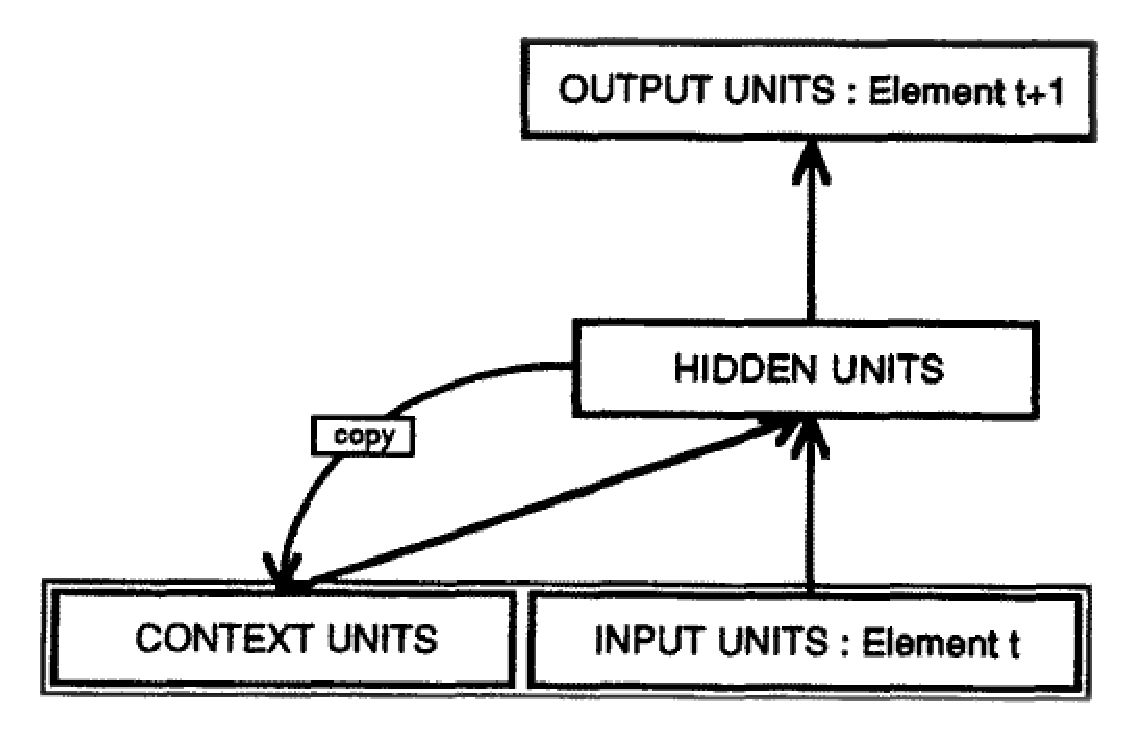
\includegraphics[width=85mm]{figures/srn.eps}
\end{center}
\caption{General structure of a Simple Recurrent Network (SRN) model.  Image adapted from Cleeremans and McClelland (1991).}
\label{SRN-Model}
\end{figure} 

\begin{figure}[t]
\begin{center}
	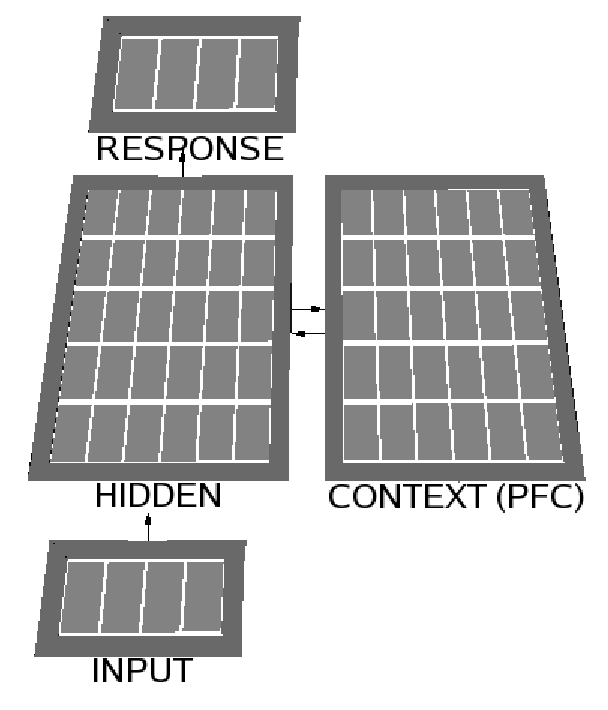
\includegraphics[width=85mm]{figures/srtt_network.eps}
\end{center}
\caption{Network Diagram of SRTT Model} 
\label{network-diagram-srtt}
\end{figure}

Since the hidden sequential structure in the intermediate blocks of the SRTT is often complex, the information provided by the context layer is vital for the success of the model.  Importantly, the context layer in this model plays an identical functional role to the PFC in other models, actively maintaining information that can be used to modulate an input-output mapping.  In our previous executive dysfunction model, the PFC actively maintained information about the currently relevant stimulus dimension (e.g., ``focus on the ink color'' in Stroop or ``sort cards based on shape'' in WCST), so as to modulate performance.  In this model, the context layer actively maintains information about the preceding button presses, allowing that information to modulate the prediction of the next button.  In our previous model, the PFC was updated in a dynamic fashion, based on learned task contingencies.  In this model, the context layer is updated with each new input presentation.  Thus, the SRN context layer is analogous to the PFC in our previous model, with the updating ``gate'' forced to open with each new input~\cite{OReillyRC:2006:MWMW}.

It is important to note that, in order to capture the relevant sequential information, the SRN must update the context layer in a fast and appropriate manner.  This flexible updating of contextual information is precisely the cognitive mechanism we hypothesize to be suspect in people with autism.  By restricting the ability of the SRN to update the context layer, mirroring the PFC updating failures that arise with weakened PFC/DA interactions in our other models, we expect to capture the performance of people with autism.

\subsubsection{Model Modifications}
We made small modifications to a previous implementation of the Cleermans SRTT model, reducing the original implementation's 10-unit inputs and outputs to only 4, to capture the structure of the 4-button SRTT~\cite{OReillyRC:2000:Computational}.  (See Figure~\ref{network-diagram-srtt}.)  In this model, an Input Layer represents the four distinct buttons.  The Hidden Layer learns the prediction mapping and provides a modeled abstraction of posterior brain systems.  A Response Layer encodes the prediction output of the network.  Additionally, a Context Layer provides a top-down influence on processing within the Hidden Layer, reflecting the role of PFC.

In order to model the performance of people with autism, we restricted the probability of successfully updating the Context Layer (PFC) upon each input presentation.  Normally, the Context Layer is updated with each input, but the autism model only updated its Context Layer with some fixed probability which was less than one.  This is analogous to reducing the efficacy of the DA-based gating signal to the PFC.  Restricting the updating of the PFC in this manner makes the temporally extended information normally contained within this layer much less reliable, making the learning of complex sequential structures much more difficult for the network.

\subsubsection{Computing Reaction Time in a SRN}
The measure of interest in the SRTT is the response time of the participants throughout the training blocks.  In order to compare model performance to human reaction times, Cleeremans et al. (1991) \nocite{Cleeremans:1991:SSRT} translated network outputs into a probability distribution over the four buttons using a Luce choice ratio~\cite{Luce:1963} and then linearly scaled the error between this prediction distribution and the actual outcome (i.e., the next button illuminated) to produce a modeled response time.  This procedure assumes that there is a linear increase in response time with prediction error.  We used this method, as well, introducing three free parameters for fitting the model to data: a linear scaling parameter from error to milliseconds, a base response time (when error is zero) for the healthy model, and a base response time for the autism model.  
%Note that different base response times were used for the normally developing and autism cases in order to capture the difficulty people with autism regularly exhibit when initiating movements~\cite{RefWorks:100}.

\subsection{Implicit Learning Simulation Results}
Network simulations were repeated 100 times in each of the experimental conditions, with initial synaptic weights randomized for each repetition.  Average performance results for each block were compared to previously reported response time data for both people with autism and normally developing controls~\cite{RefWorks:148}.  The updating probability, and associated scaling parameters, that produced the lowest sum-squared deviation from the human data was identified as the best fit model.

The simulation results match human performance both qualitatively and quantitatively, providing evidence that impairments in PFC updating can result in implicit learning deficits like those seen in people with autism.  When the healthy network is restricted to perfectly update its Context Layer (i.e., with probability one), the corresponding best-fit probability for the autism network is $0.5$, with an SSE of $652$. The corresponding scaling parameter from error to reaction time is $261.4$, the healthy base time is $458.6$ msec, and the autism base time is $534.5$ msec.  The resulting modeled reaction times, along with human data from the literature, is shown in Figure~\ref{Model-Results}.

\begin{figure}[t]
\begin{center}
%%	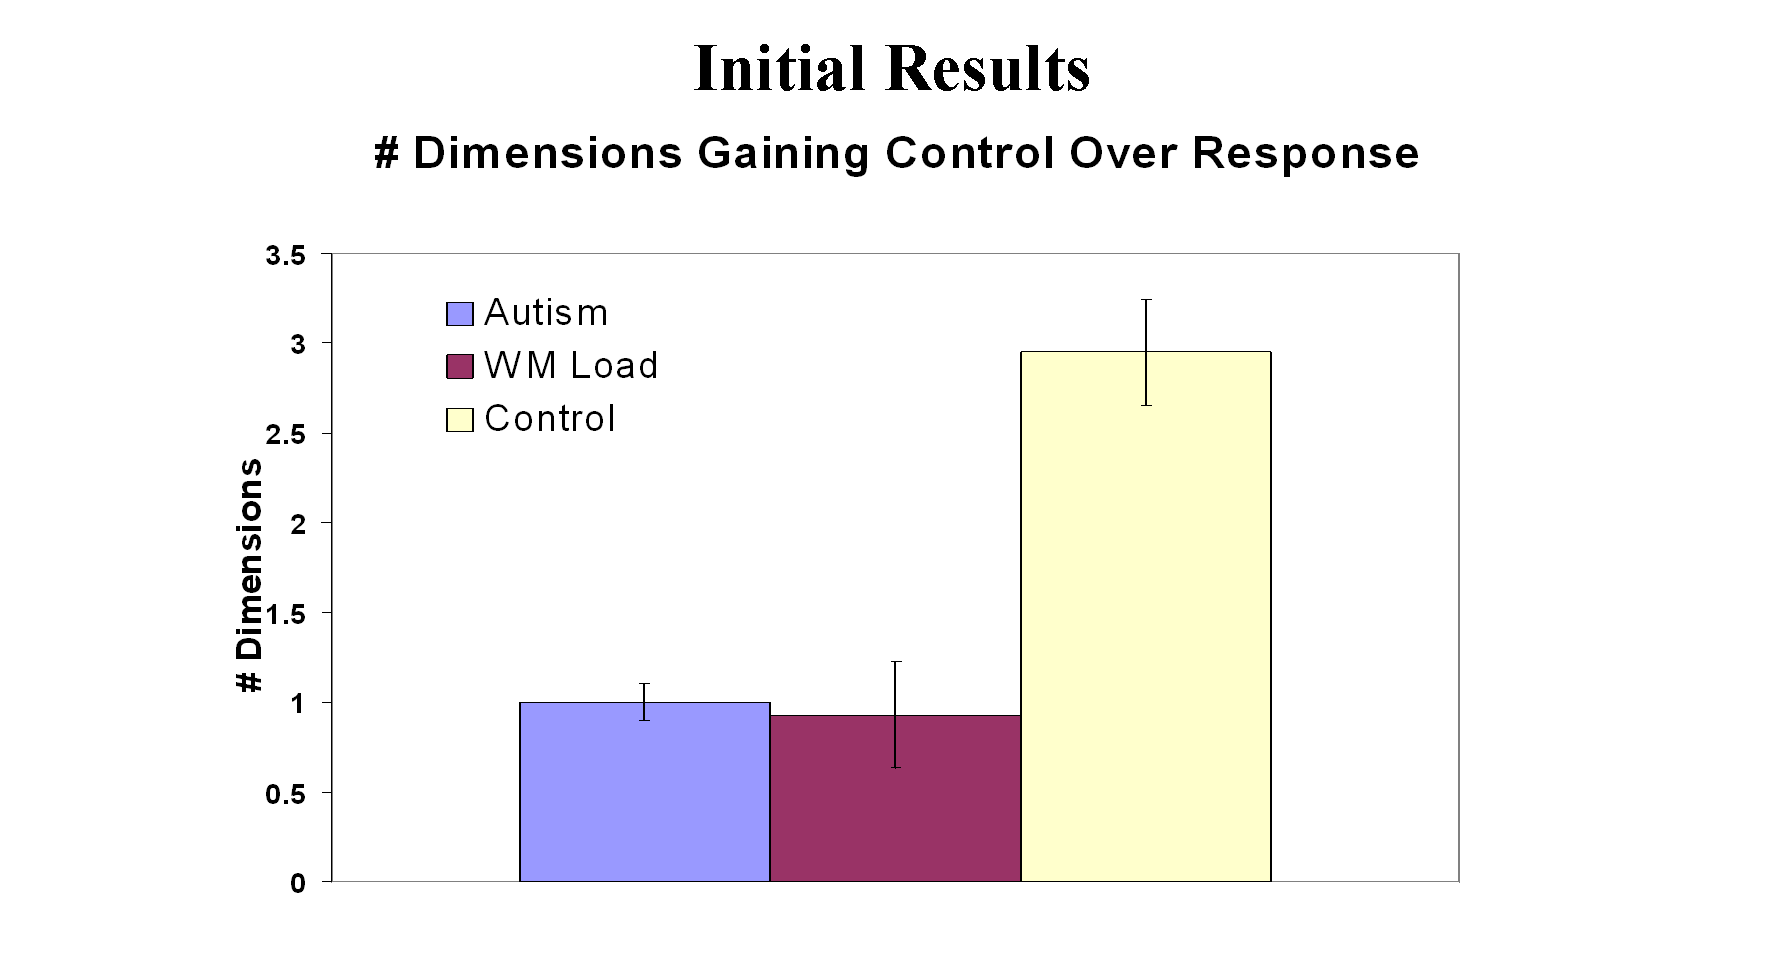
\includegraphics[width=125mm]{graphs/OS_initial_results.eps}
	\includegraphics[width=115mm]{graphs/srtt_chart.ps}
\end{center}
\caption{Scaled Model Results \& Human Behavioral Data from Mostofsky
         et al. (2000)} 
\label{Model-Results}
\end{figure} 

A repeated measures ANOVA was conducted on blocks 1, 2, 3, and 4 of the model results, and a significant Group by Block interaction ($F(3, 97) = 62.007$; $p < 0.000001$) was detected. From these results we can conclude that the networks simulating autistic performance demonstrated significantly less learning over the crucial training blocks of 2, 3, and 4, as compared to the networks allowed to properly update their PFC-like Context Layers.  Thus, clear implicit learning deficits were present in the autism model.

%The modeling results presented in this section suggest that, in people with autism, implicit learning deficits may be driven largely by abnormalities in DA/PFC interactions, causing inflexibility in the updating of contextual information.  Without the proper updating of actively maintained contextual information, it is essentially impossible to properly integrate temporally separated pieces of information, such as the order of items in a sequence.  Thus, our computational account highlights how PFC/DA dysfunction can lead to problems with information integration.  This is particularly interesting, since one prominent behavioral theory of autism, \emph{Weak Central Coherence}, posits that deficits in integrating contextual information lay at the core of this disorder~\cite{HappeF:1999:WCC}.  
